\documentclass{book}

\usepackage[spanish]{babel}
\usepackage[utf8]{inputenc}
\usepackage[T1]{fontenc}

\usepackage[
  top=3cm,
  bottom=3cm,
  left=2cm,
  right=2cm,
  heightrounded,
]{geometry}

\author{Bruno Martinez}
\title{Bruno}
\date{\today}

\begin{document}

\maketitle

\chapter*{Introducción}

\chapter{Bruno}

Plantilla de \large{\LaTex.}

\section{un poco sobre mí}

Me llamo Bruno, nací en la CDMX (cuando aún era DF) y he vivido aquí mis 18 as de vida. 


\section{hobbies}
\begin{itemize}
\item Jugar fútbol.
\item Jugar videojuegos
\item Ver televisión.
\end {itemize}

\newpage
Algunas formulas importantes en mi vida son:
\begin{itemize}
\item $c² = a² + b²$
\item $x=-b \pm \frac{\sqrt{b²-4ac}}{2a}$
\end{itemize}

\section{algo de matemáticas simples}
\begin{figure}[h]
  \centering
  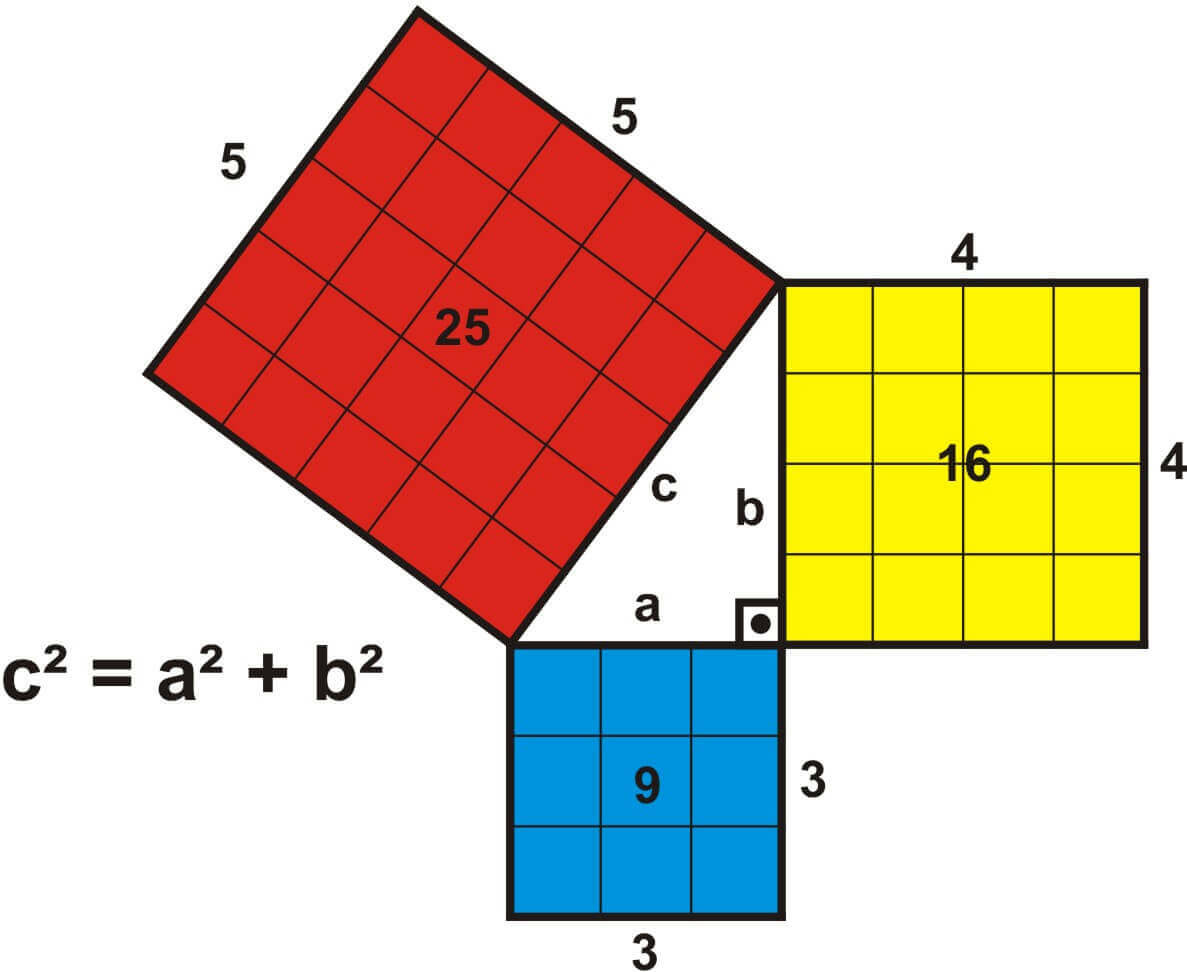
\includegraphics[scale=0.5]{IMG/pitagoras.jpg}
  \caption{Imagen sobre el teorema de Pitágoras}
  \label{fig:Pitágoras}
\end{figure}

Podemos ver un ejemplo del \emph{Teorema de Pitágoras} en la \emph{\textbf{Figura}}~\ref{fig:pitagoras}
  
\bibliographystyle{acm}
\bibliography{bibliografía}

\end{document}
